\documentclass[1p]{elsarticle_modified}
%\bibliographystyle{elsarticle-num}

%\usepackage[colorlinks]{hyperref}
%\usepackage{abbrmath_seonhwa} %\Abb, \Ascr, \Acal ,\Abf, \Afrak
\usepackage{amsfonts}
\usepackage{amssymb}
\usepackage{amsmath}
\usepackage{amsthm}
\usepackage{scalefnt}
\usepackage{amsbsy}
\usepackage{kotex}
\usepackage{caption}
\usepackage{subfig}
\usepackage{color}
\usepackage{graphicx}
\usepackage{xcolor} %% white, black, red, green, blue, cyan, magenta, yellow
\usepackage{float}
\usepackage{setspace}
\usepackage{hyperref}

\usepackage{tikz}
\usetikzlibrary{arrows}

\usepackage{multirow}
\usepackage{array} % fixed length table
\usepackage{hhline}

%%%%%%%%%%%%%%%%%%%%%
\makeatletter
\renewcommand*\env@matrix[1][\arraystretch]{%
	\edef\arraystretch{#1}%
	\hskip -\arraycolsep
	\let\@ifnextchar\new@ifnextchar
	\array{*\c@MaxMatrixCols c}}
\makeatother %https://tex.stackexchange.com/questions/14071/how-can-i-increase-the-line-spacing-in-a-matrix
%%%%%%%%%%%%%%%

\usepackage[normalem]{ulem}

\newcommand{\msout}[1]{\ifmmode\text{\sout{\ensuremath{#1}}}\else\sout{#1}\fi}
%SOURCE: \msout is \stkout macro in https://tex.stackexchange.com/questions/20609/strikeout-in-math-mode

\newcommand{\cancel}[1]{
	\ifmmode
	{\color{red}\msout{#1}}
	\else
	{\color{red}\sout{#1}}
	\fi
}

\newcommand{\add}[1]{
	{\color{blue}\uwave{#1}}
}

\newcommand{\replace}[2]{
	\ifmmode
	{\color{red}\msout{#1}}{\color{blue}\uwave{#2}}
	\else
	{\color{red}\sout{#1}}{\color{blue}\uwave{#2}}
	\fi
}

\newcommand{\Sol}{\mathcal{S}} %segment
\newcommand{\D}{D} %diagram
\newcommand{\A}{\mathcal{A}} %arc


%%%%%%%%%%%%%%%%%%%%%%%%%%%%%5 test

\def\sl{\operatorname{\textup{SL}}(2,\Cbb)}
\def\psl{\operatorname{\textup{PSL}}(2,\Cbb)}
\def\quan{\mkern 1mu \triangleright \mkern 1mu}

\theoremstyle{definition}
\newtheorem{thm}{Theorem}[section]
\newtheorem{prop}[thm]{Proposition}
\newtheorem{lem}[thm]{Lemma}
\newtheorem{ques}[thm]{Question}
\newtheorem{cor}[thm]{Corollary}
\newtheorem{defn}[thm]{Definition}
\newtheorem{exam}[thm]{Example}
\newtheorem{rmk}[thm]{Remark}
\newtheorem{alg}[thm]{Algorithm}

\newcommand{\I}{\sqrt{-1}}
\begin{document}

%\begin{frontmatter}
%
%\title{Boundary parabolic representations of knots up to 8 crossings}
%
%%% Group authors per affiliation:
%\author{Yunhi Cho} 
%\address{Department of Mathematics, University of Seoul, Seoul, Korea}
%\ead{yhcho@uos.ac.kr}
%
%
%\author{Seonhwa Kim} %\fnref{s_kim}}
%\address{Center for Geometry and Physics, Institute for Basic Science, Pohang, 37673, Korea}
%\ead{ryeona17@ibs.re.kr}
%
%\author{Hyuk Kim}
%\address{Department of Mathematical Sciences, Seoul National University, Seoul 08826, Korea}
%\ead{hyukkim@snu.ac.kr}
%
%\author{Seokbeom Yoon}
%\address{Department of Mathematical Sciences, Seoul National University, Seoul, 08826,  Korea}
%\ead{sbyoon15@snu.ac.kr}
%
%\begin{abstract}
%We find all boundary parabolic representation of knots up to 8 crossings.
%
%\end{abstract}
%\begin{keyword}
%    \MSC[2010] 57M25 
%\end{keyword}
%
%\end{frontmatter}

%\linenumbers
%\tableofcontents
%
\newcommand\colored[1]{\textcolor{white}{\rule[-0.35ex]{0.8em}{1.4ex}}\kern-0.8em\color{red} #1}%
%\newcommand\colored[1]{\textcolor{white}{ #1}\kern-2.17ex	\textcolor{white}{ #1}\kern-1.81ex	\textcolor{white}{ #1}\kern-2.15ex\color{red}#1	}

{\Large $\underline{12n_{0768}~(K12n_{0768})}$}

\setlength{\tabcolsep}{10pt}
\renewcommand{\arraystretch}{1.6}
\vspace{1cm}\begin{tabular}{m{100pt}>{\centering\arraybackslash}m{274pt}}
\multirow{5}{120pt}{
	\centering
	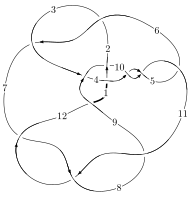
\includegraphics[width=112pt]{../../../GIT/diagram.site/Diagrams/png/2857_12n_0768.png}\\
\ \ \ A knot diagram\footnotemark}&
\allowdisplaybreaks
\textbf{Linearized knot diagam} \\
\cline{2-2}
 &
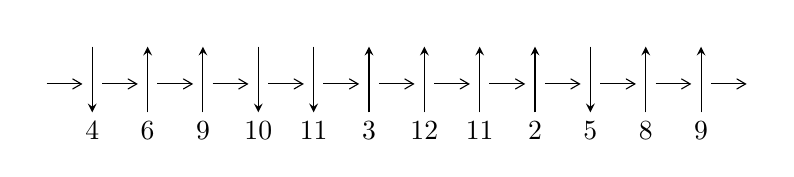
\begin{tikzpicture}[x=20pt, y=17pt]
	% nodes
	\node (C0) at (0, 0) {};
	\node (C1) at (1, 0) {};
	\node (C1U) at (1, +1) {};
	\node (C1D) at (1, -1) {4};

	\node (C2) at (2, 0) {};
	\node (C2U) at (2, +1) {};
	\node (C2D) at (2, -1) {6};

	\node (C3) at (3, 0) {};
	\node (C3U) at (3, +1) {};
	\node (C3D) at (3, -1) {9};

	\node (C4) at (4, 0) {};
	\node (C4U) at (4, +1) {};
	\node (C4D) at (4, -1) {10};

	\node (C5) at (5, 0) {};
	\node (C5U) at (5, +1) {};
	\node (C5D) at (5, -1) {11};

	\node (C6) at (6, 0) {};
	\node (C6U) at (6, +1) {};
	\node (C6D) at (6, -1) {3};

	\node (C7) at (7, 0) {};
	\node (C7U) at (7, +1) {};
	\node (C7D) at (7, -1) {12};

	\node (C8) at (8, 0) {};
	\node (C8U) at (8, +1) {};
	\node (C8D) at (8, -1) {11};

	\node (C9) at (9, 0) {};
	\node (C9U) at (9, +1) {};
	\node (C9D) at (9, -1) {2};

	\node (C10) at (10, 0) {};
	\node (C10U) at (10, +1) {};
	\node (C10D) at (10, -1) {5};

	\node (C11) at (11, 0) {};
	\node (C11U) at (11, +1) {};
	\node (C11D) at (11, -1) {8};

	\node (C12) at (12, 0) {};
	\node (C12U) at (12, +1) {};
	\node (C12D) at (12, -1) {9};
	\node (C13) at (13, 0) {};

	% arrows
	\draw[->,>={angle 60}]
	(C0) edge (C1) (C1) edge (C2) (C2) edge (C3) (C3) edge (C4) (C4) edge (C5) (C5) edge (C6) (C6) edge (C7) (C7) edge (C8) (C8) edge (C9) (C9) edge (C10) (C10) edge (C11) (C11) edge (C12) (C12) edge (C13) ;	\draw[->,>=stealth]
	(C1U) edge (C1D) (C2D) edge (C2U) (C3D) edge (C3U) (C4U) edge (C4D) (C5U) edge (C5D) (C6D) edge (C6U) (C7D) edge (C7U) (C8D) edge (C8U) (C9D) edge (C9U) (C10U) edge (C10D) (C11D) edge (C11U) (C12D) edge (C12U) ;
	\end{tikzpicture} \\
\hhline{~~} \\& 
\textbf{Solving Sequence} \\ \cline{2-2} 
 &
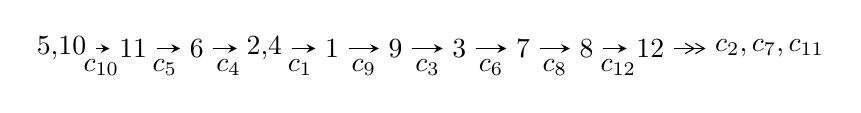
\begin{tikzpicture}[x=23pt, y=7pt]
	% node
	\node (A0) at (-1/8, 0) {5,10};
	\node (A1) at (1, 0) {11};
	\node (A2) at (2, 0) {6};
	\node (A3) at (49/16, 0) {2,4};
	\node (A4) at (33/8, 0) {1};
	\node (A5) at (41/8, 0) {9};
	\node (A6) at (49/8, 0) {3};
	\node (A7) at (57/8, 0) {7};
	\node (A8) at (65/8, 0) {8};
	\node (A9) at (73/8, 0) {12};
	\node (C1) at (1/2, -1) {$c_{10}$};
	\node (C2) at (3/2, -1) {$c_{5}$};
	\node (C3) at (5/2, -1) {$c_{4}$};
	\node (C4) at (29/8, -1) {$c_{1}$};
	\node (C5) at (37/8, -1) {$c_{9}$};
	\node (C6) at (45/8, -1) {$c_{3}$};
	\node (C7) at (53/8, -1) {$c_{6}$};
	\node (C8) at (61/8, -1) {$c_{8}$};
	\node (C9) at (69/8, -1) {$c_{12}$};
	\node (A10) at (11, 0) {$c_{2},c_{7},c_{11}$};

	% edge
	\draw[->,>=stealth]	
	(A0) edge (A1) (A1) edge (A2) (A2) edge (A3) (A3) edge (A4) (A4) edge (A5) (A5) edge (A6) (A6) edge (A7) (A7) edge (A8) (A8) edge (A9) ;
	\draw[->>,>={angle 60}]	
	(A9) edge (A10);
\end{tikzpicture} \\ 

\end{tabular} \\

\footnotetext{
The image of knot diagram is generated by the software ``\textbf{Draw programme}" developed by Andrew Bartholomew(\url{http://www.layer8.co.uk/maths/draw/index.htm\#Running-draw}), where we modified some parts for our purpose(\url{https://github.com/CATsTAILs/LinksPainter}).
}\phantom \\ \newline 
\centering \textbf{Ideals for irreducible components\footnotemark of $X_{\text{par}}$} 
 
\begin{align*}
I^u_{1}&=\langle 
-2.92778\times10^{21} u^{25}+2.56531\times10^{22} u^{24}+\cdots+3.87990\times10^{23} b-1.26738\times10^{24},\\
\phantom{I^u_{1}}&\phantom{= \langle  }2.71108\times10^{23} u^{25}+1.09424\times10^{24} u^{24}+\cdots+1.20277\times10^{25} a-1.27374\times10^{26},\;u^{26}- u^{25}+\cdots+12 u+31\rangle \\
I^u_{2}&=\langle 
- u^{13}+6 u^{11}+u^{10}-14 u^9-6 u^8+14 u^7+15 u^6-3 u^5-18 u^4-5 u^3+9 u^2+b+3 u-1,\\
\phantom{I^u_{2}}&\phantom{= \langle  }- u^{13}+u^{12}+6 u^{11}-4 u^{10}-15 u^9+2 u^8+19 u^7+13 u^6-12 u^5-22 u^4+10 u^2+a+5 u-1,\\
\phantom{I^u_{2}}&\phantom{= \langle  }u^{14}-7 u^{12}- u^{11}+19 u^{10}+7 u^9-23 u^8-20 u^7+8 u^6+28 u^5+7 u^4-17 u^3-6 u^2+2 u+1\rangle \\
\\
\end{align*}
\raggedright * 2 irreducible components of $\dim_{\mathbb{C}}=0$, with total 40 representations.\\
\footnotetext{All coefficients of polynomials are rational numbers. But the coefficients are sometimes approximated in decimal forms when there is not enough margin.}
\newpage
\renewcommand{\arraystretch}{1}
\centering \section*{I. $I^u_{1}= \langle -2.93\times10^{21} u^{25}+2.57\times10^{22} u^{24}+\cdots+3.88\times10^{23} b-1.27\times10^{24},\;2.71\times10^{23} u^{25}+1.09\times10^{24} u^{24}+\cdots+1.20\times10^{25} a-1.27\times10^{26},\;u^{26}- u^{25}+\cdots+12 u+31 \rangle$}
\flushleft \textbf{(i) Arc colorings}\\
\begin{tabular}{m{7pt} m{180pt} m{7pt} m{180pt} }
\flushright $a_{5}=$&$\begin{pmatrix}0\\u\end{pmatrix}$ \\
\flushright $a_{10}=$&$\begin{pmatrix}1\\0\end{pmatrix}$ \\
\flushright $a_{11}=$&$\begin{pmatrix}1\\u^2\end{pmatrix}$ \\
\flushright $a_{6}=$&$\begin{pmatrix}- u\\- u^3+u\end{pmatrix}$ \\
\flushright $a_{2}=$&$\begin{pmatrix}-0.0225403 u^{25}-0.0909766 u^{24}+\cdots+5.26309 u+10.5900\\0.00754601 u^{25}-0.0661178 u^{24}+\cdots-2.55257 u+3.26654\end{pmatrix}$ \\
\flushright $a_{4}=$&$\begin{pmatrix}u\\u\end{pmatrix}$ \\
\flushright $a_{1}=$&$\begin{pmatrix}-0.0460308 u^{25}-0.0975533 u^{24}+\cdots+3.67107 u+8.88673\\-0.0159445 u^{25}-0.0726945 u^{24}+\cdots-4.14458 u+1.56324\end{pmatrix}$ \\
\flushright $a_{9}=$&$\begin{pmatrix}-0.0228681 u^{25}-0.107777 u^{24}+\cdots-0.424141 u+6.30289\\0.105094 u^{25}-0.0463805 u^{24}+\cdots-7.82285 u-2.16744\end{pmatrix}$ \\
\flushright $a_{3}=$&$\begin{pmatrix}-0.0714029 u^{25}-0.131292 u^{24}+\cdots+7.63526 u+15.5015\\0.00756581 u^{25}-0.0451761 u^{24}+\cdots-2.33987 u+1.11953\end{pmatrix}$ \\
\flushright $a_{7}=$&$\begin{pmatrix}-0.466848 u^{25}+0.229048 u^{24}+\cdots+25.8666 u+8.47181\\0.0444585 u^{25}+0.0166367 u^{24}+\cdots-2.65167 u-3.76153\end{pmatrix}$ \\
\flushright $a_{8}=$&$\begin{pmatrix}-0.192283 u^{25}-0.0910018 u^{24}+\cdots+9.67536 u+12.5203\\-0.00596389 u^{25}-0.0322573 u^{24}+\cdots-0.739325 u+2.56438\end{pmatrix}$ \\
\flushright $a_{12}=$&$\begin{pmatrix}0.235482 u^{25}-0.154199 u^{24}+\cdots-20.6106 u-7.26827\\0.0223603 u^{25}-0.0205281 u^{24}+\cdots-3.27390 u-0.0676271\end{pmatrix}$\\&\end{tabular}
\flushleft \textbf{(ii) Obstruction class $= -1$}\\~\\
\flushleft \textbf{(iii) Cusp Shapes $= -\frac{46652502203510047014961}{129330126954099989822173} u^{25}+\frac{99744336497876668876271}{387990380862299969466519} u^{24}+\cdots+\frac{7467042075154247618912122}{387990380862299969466519} u-\frac{1919651047154391762384890}{387990380862299969466519}$}\\~\\
\newpage\renewcommand{\arraystretch}{1}
\flushleft \textbf{(iv) u-Polynomials at the component}\newline \\
\begin{tabular}{m{50pt}|m{274pt}}
Crossings & \hspace{64pt}u-Polynomials at each crossing \\
\hline $$\begin{aligned}c_{1}\end{aligned}$$&$\begin{aligned}
&u^{26}-24 u^{24}+\cdots-352 u+41
\end{aligned}$\\
\hline $$\begin{aligned}c_{2},c_{6}\end{aligned}$$&$\begin{aligned}
&u^{26}-4 u^{25}+\cdots-322 u-529
\end{aligned}$\\
\hline $$\begin{aligned}c_{3}\end{aligned}$$&$\begin{aligned}
&u^{26}- u^{25}+\cdots-12769 u-1781
\end{aligned}$\\
\hline $$\begin{aligned}c_{4},c_{5},c_{10}\end{aligned}$$&$\begin{aligned}
&u^{26}+u^{25}+\cdots-12 u+31
\end{aligned}$\\
\hline $$\begin{aligned}c_{7},c_{8},c_{11}\end{aligned}$$&$\begin{aligned}
&u^{26}+u^{25}+\cdots-34 u-4
\end{aligned}$\\
\hline $$\begin{aligned}c_{9}\end{aligned}$$&$\begin{aligned}
&u^{26}+2 u^{25}+\cdots+36 u-19
\end{aligned}$\\
\hline $$\begin{aligned}c_{12}\end{aligned}$$&$\begin{aligned}
&u^{26}- u^{25}+\cdots-304218 u-40564
\end{aligned}$\\
\hline
\end{tabular}\\~\\
\newpage\renewcommand{\arraystretch}{1}
\flushleft \textbf{(v) Riley Polynomials at the component}\newline \\
\begin{tabular}{m{50pt}|m{274pt}}
Crossings & \hspace{64pt}Riley Polynomials at each crossing \\
\hline $$\begin{aligned}c_{1}\end{aligned}$$&$\begin{aligned}
&y^{26}-48 y^{25}+\cdots+19924 y+1681
\end{aligned}$\\
\hline $$\begin{aligned}c_{2},c_{6}\end{aligned}$$&$\begin{aligned}
&y^{26}+12 y^{25}+\cdots-348082 y+279841
\end{aligned}$\\
\hline $$\begin{aligned}c_{3}\end{aligned}$$&$\begin{aligned}
&y^{26}+69 y^{25}+\cdots-266466469 y+3171961
\end{aligned}$\\
\hline $$\begin{aligned}c_{4},c_{5},c_{10}\end{aligned}$$&$\begin{aligned}
&y^{26}-33 y^{25}+\cdots-12482 y+961
\end{aligned}$\\
\hline $$\begin{aligned}c_{7},c_{8},c_{11}\end{aligned}$$&$\begin{aligned}
&y^{26}+43 y^{25}+\cdots-716 y+16
\end{aligned}$\\
\hline $$\begin{aligned}c_{9}\end{aligned}$$&$\begin{aligned}
&y^{26}+6 y^{25}+\cdots+1782 y+361
\end{aligned}$\\
\hline $$\begin{aligned}c_{12}\end{aligned}$$&$\begin{aligned}
&y^{26}+147 y^{25}+\cdots-80260701260 y+1645438096
\end{aligned}$\\
\hline
\end{tabular}\\~\\
\newpage\flushleft \textbf{(vi) Complex Volumes and Cusp Shapes}
$$\begin{array}{c|c|c}  
\text{Solutions to }I^u_{1}& \I (\text{vol} + \sqrt{-1}CS) & \text{Cusp shape}\\
 \hline 
\begin{aligned}
u &= \phantom{-}0.764982 + 0.335496 I \\
a &= \phantom{-}0.043942 - 0.279919 I \\
b &= \phantom{-}1.019140 - 0.401366 I\end{aligned}
 & -1.38320 - 3.64635 I & \phantom{-}1.35824 + 7.32767 I \\ \hline\begin{aligned}
u &= \phantom{-}0.764982 - 0.335496 I \\
a &= \phantom{-}0.043942 + 0.279919 I \\
b &= \phantom{-}1.019140 + 0.401366 I\end{aligned}
 & -1.38320 + 3.64635 I & \phantom{-}1.35824 - 7.32767 I \\ \hline\begin{aligned}
u &= \phantom{-}0.777607 + 0.118039 I \\
a &= \phantom{-}2.55907 - 0.95852 I \\
b &= -0.478055 - 0.742412 I\end{aligned}
 & -13.15060 - 0.37776 I & -1.22408 - 1.34498 I \\ \hline\begin{aligned}
u &= \phantom{-}0.777607 - 0.118039 I \\
a &= \phantom{-}2.55907 + 0.95852 I \\
b &= -0.478055 + 0.742412 I\end{aligned}
 & -13.15060 + 0.37776 I & -1.22408 + 1.34498 I \\ \hline\begin{aligned}
u &= \phantom{-}0.842907 + 0.881469 I \\
a &= -0.571747 + 0.134450 I \\
b &= -0.469429 - 0.674553 I\end{aligned}
 & -1.203930 - 0.496037 I & \phantom{-}0.79686 - 2.54300 I \\ \hline\begin{aligned}
u &= \phantom{-}0.842907 - 0.881469 I \\
a &= -0.571747 - 0.134450 I \\
b &= -0.469429 + 0.674553 I\end{aligned}
 & -1.203930 + 0.496037 I & \phantom{-}0.79686 + 2.54300 I \\ \hline\begin{aligned}
u &= -0.719777\phantom{ +0.000000I} \\
a &= -0.187725\phantom{ +0.000000I} \\
b &= -1.16272\phantom{ +0.000000I}\end{aligned}
 & \phantom{-}2.17524\phantom{ +0.000000I} & \phantom{-}2.79410\phantom{ +0.000000I} \\ \hline\begin{aligned}
u &= \phantom{-}0.159981 + 0.568954 I \\
a &= \phantom{-}0.445478 + 0.461168 I \\
b &= -0.321692 + 0.362997 I\end{aligned}
 & \phantom{-}0.333623 - 1.008960 I & \phantom{-}5.28376 + 6.66934 I \\ \hline\begin{aligned}
u &= \phantom{-}0.159981 - 0.568954 I \\
a &= \phantom{-}0.445478 - 0.461168 I \\
b &= -0.321692 - 0.362997 I\end{aligned}
 & \phantom{-}0.333623 + 1.008960 I & \phantom{-}5.28376 - 6.66934 I \\ \hline\begin{aligned}
u &= -1.40068 + 0.23284 I \\
a &= -0.23778 + 1.47903 I \\
b &= \phantom{-}0.413279 + 0.877413 I\end{aligned}
 & -4.79645 + 4.01069 I & \phantom{-}0.34699 - 9.12487 I\\
 \hline 
 \end{array}$$\newpage$$\begin{array}{c|c|c}  
\text{Solutions to }I^u_{1}& \I (\text{vol} + \sqrt{-1}CS) & \text{Cusp shape}\\
 \hline 
\begin{aligned}
u &= -1.40068 - 0.23284 I \\
a &= -0.23778 - 1.47903 I \\
b &= \phantom{-}0.413279 - 0.877413 I\end{aligned}
 & -4.79645 - 4.01069 I & \phantom{-}0.34699 + 9.12487 I \\ \hline\begin{aligned}
u &= -0.571043\phantom{ +0.000000I} \\
a &= \phantom{-}2.07972\phantom{ +0.000000I} \\
b &= \phantom{-}0.907867\phantom{ +0.000000I}\end{aligned}
 & \phantom{-}2.93787\phantom{ +0.000000I} & -5.61080\phantom{ +0.000000I} \\ \hline\begin{aligned}
u &= -0.484610 + 0.243441 I \\
a &= -1.71290 + 0.53126 I \\
b &= \phantom{-}0.461065 + 0.861987 I\end{aligned}
 & -3.51192 + 0.62346 I & -2.84586 - 0.67416 I \\ \hline\begin{aligned}
u &= -0.484610 - 0.243441 I \\
a &= -1.71290 - 0.53126 I \\
b &= \phantom{-}0.461065 - 0.861987 I\end{aligned}
 & -3.51192 - 0.62346 I & -2.84586 + 0.67416 I \\ \hline\begin{aligned}
u &= \phantom{-}1.52698 + 0.20871 I \\
a &= \phantom{-}0.133555 + 1.387270 I \\
b &= -1.051380 + 0.928731 I\end{aligned}
 & -10.29450 - 2.62985 I & -1.70383 + 1.78381 I \\ \hline\begin{aligned}
u &= \phantom{-}1.52698 - 0.20871 I \\
a &= \phantom{-}0.133555 - 1.387270 I \\
b &= -1.051380 - 0.928731 I\end{aligned}
 & -10.29450 + 2.62985 I & -1.70383 - 1.78381 I \\ \hline\begin{aligned}
u &= -0.82721 + 1.33251 I \\
a &= \phantom{-}0.352400 - 0.194950 I \\
b &= -0.445225 - 1.242010 I\end{aligned}
 & -15.2105 + 4.3640 I & -1.41577 - 3.17462 I \\ \hline\begin{aligned}
u &= -0.82721 - 1.33251 I \\
a &= \phantom{-}0.352400 + 0.194950 I \\
b &= -0.445225 + 1.242010 I\end{aligned}
 & -15.2105 - 4.3640 I & -1.41577 + 3.17462 I \\ \hline\begin{aligned}
u &= \phantom{-}1.65746 + 0.14713 I \\
a &= \phantom{-}0.159581 + 0.992092 I \\
b &= \phantom{-}0.250667 + 1.107520 I\end{aligned}
 & -5.67875 - 1.02437 I & -0.521896 - 0.910763 I \\ \hline\begin{aligned}
u &= \phantom{-}1.65746 - 0.14713 I \\
a &= \phantom{-}0.159581 - 0.992092 I \\
b &= \phantom{-}0.250667 - 1.107520 I\end{aligned}
 & -5.67875 + 1.02437 I & -0.521896 + 0.910763 I\\
 \hline 
 \end{array}$$\newpage$$\begin{array}{c|c|c}  
\text{Solutions to }I^u_{1}& \I (\text{vol} + \sqrt{-1}CS) & \text{Cusp shape}\\
 \hline 
\begin{aligned}
u &= -1.77337 + 0.06842 I \\
a &= \phantom{-}0.294799 - 0.960179 I \\
b &= \phantom{-}1.44079 - 1.23613 I\end{aligned}
 & \phantom{-}16.7710 + 1.3129 I & -1.252333 - 0.225172 I \\ \hline\begin{aligned}
u &= -1.77337 - 0.06842 I \\
a &= \phantom{-}0.294799 + 0.960179 I \\
b &= \phantom{-}1.44079 + 1.23613 I\end{aligned}
 & \phantom{-}16.7710 - 1.3129 I & -1.252333 + 0.225172 I \\ \hline\begin{aligned}
u &= \phantom{-}1.74642 + 0.44620 I \\
a &= -0.080704 - 1.254640 I \\
b &= \phantom{-}1.18154 - 1.35502 I\end{aligned}
 & \phantom{-}16.0643 - 11.0020 I & -1.09431 + 4.10898 I \\ \hline\begin{aligned}
u &= \phantom{-}1.74642 - 0.44620 I \\
a &= -0.080704 + 1.254640 I \\
b &= \phantom{-}1.18154 + 1.35502 I\end{aligned}
 & \phantom{-}16.0643 + 11.0020 I & -1.09431 - 4.10898 I \\ \hline\begin{aligned}
u &= -1.84505 + 0.14739 I \\
a &= -0.154266 - 1.018760 I \\
b &= -0.87327 - 1.36223 I\end{aligned}
 & -11.74950 + 5.10402 I & -1.81943 - 2.88501 I \\ \hline\begin{aligned}
u &= -1.84505 - 0.14739 I \\
a &= -0.154266 + 1.018760 I \\
b &= -0.87327 + 1.36223 I\end{aligned}
 & -11.74950 - 5.10402 I & -1.81943 + 2.88501 I\\
 \hline 
 \end{array}$$\newpage\newpage\renewcommand{\arraystretch}{1}
\centering \section*{II. $I^u_{2}= \langle - u^{13}+6 u^{11}+\cdots+b-1,\;- u^{13}+u^{12}+\cdots+a-1,\;u^{14}-7 u^{12}+\cdots+2 u+1 \rangle$}
\flushleft \textbf{(i) Arc colorings}\\
\begin{tabular}{m{7pt} m{180pt} m{7pt} m{180pt} }
\flushright $a_{5}=$&$\begin{pmatrix}0\\u\end{pmatrix}$ \\
\flushright $a_{10}=$&$\begin{pmatrix}1\\0\end{pmatrix}$ \\
\flushright $a_{11}=$&$\begin{pmatrix}1\\u^2\end{pmatrix}$ \\
\flushright $a_{6}=$&$\begin{pmatrix}- u\\- u^3+u\end{pmatrix}$ \\
\flushright $a_{2}=$&$\begin{pmatrix}u^{13}- u^{12}+\cdots-5 u+1\\u^{13}-6 u^{11}+\cdots-3 u+1\end{pmatrix}$ \\
\flushright $a_{4}=$&$\begin{pmatrix}u\\u\end{pmatrix}$ \\
\flushright $a_{1}=$&$\begin{pmatrix}u^{13}+u^{12}+\cdots-4 u^2-7 u\\u^{13}+2 u^{12}+\cdots-3 u^2-5 u\end{pmatrix}$ \\
\flushright $a_{9}=$&$\begin{pmatrix}- u^{13}+2 u^{12}+\cdots+10 u^3+3\\2 u^{12}- u^{11}+\cdots- u+1\end{pmatrix}$ \\
\flushright $a_{3}=$&$\begin{pmatrix}u^{13}-6 u^{11}+\cdots-5 u^2-8 u\\u^{13}-6 u^{11}+\cdots-2 u+1\end{pmatrix}$ \\
\flushright $a_{7}=$&$\begin{pmatrix}u^{13}-5 u^{11}- u^{10}+8 u^9+4 u^8- u^7-5 u^6-6 u^5- u^3+3 u^2+6 u\\u^{12}+u^{11}+\cdots+u-2\end{pmatrix}$ \\
\flushright $a_{8}=$&$\begin{pmatrix}-3 u^{13}+4 u^{12}+\cdots+20 u^2-2 u\\-2 u^{13}+5 u^{12}+\cdots-3 u-1\end{pmatrix}$ \\
\flushright $a_{12}=$&$\begin{pmatrix}-4 u^{13}+5 u^{12}+\cdots-5 u-7\\-3 u^{13}+6 u^{12}+\cdots-8 u-4\end{pmatrix}$\\&\end{tabular}
\flushleft \textbf{(ii) Obstruction class $= 1$}\\~\\
\flushleft \textbf{(iii) Cusp Shapes $= -2 u^{13}-3 u^{12}+16 u^{11}+20 u^{10}-44 u^9-56 u^8+40 u^7+84 u^6+28 u^5-71 u^4-68 u^3+24 u^2+27 u+7$}\\~\\
\newpage\renewcommand{\arraystretch}{1}
\flushleft \textbf{(iv) u-Polynomials at the component}\newline \\
\begin{tabular}{m{50pt}|m{274pt}}
Crossings & \hspace{64pt}u-Polynomials at each crossing \\
\hline $$\begin{aligned}c_{1}\end{aligned}$$&$\begin{aligned}
&u^{14}-5 u^{13}+\cdots- u^2+1
\end{aligned}$\\
\hline $$\begin{aligned}c_{2}\end{aligned}$$&$\begin{aligned}
&u^{14}-3 u^{13}+8 u^{11}-9 u^{10}+13 u^8-16 u^7+14 u^5-9 u^4-3 u^3+4 u^2-1
\end{aligned}$\\
\hline $$\begin{aligned}c_{3}\end{aligned}$$&$\begin{aligned}
&u^{14}+4 u^{12}+5 u^{10}+2 u^9-3 u^8+4 u^7- u^6- u^5+u^4+2 u^3+u^2- u-1
\end{aligned}$\\
\hline $$\begin{aligned}c_{4},c_{5}\end{aligned}$$&$\begin{aligned}
&u^{14}-7 u^{12}+\cdots-2 u+1
\end{aligned}$\\
\hline $$\begin{aligned}c_{6}\end{aligned}$$&$\begin{aligned}
&u^{14}+3 u^{13}-8 u^{11}-9 u^{10}+13 u^8+16 u^7-14 u^5-9 u^4+3 u^3+4 u^2-1
\end{aligned}$\\
\hline $$\begin{aligned}c_{7},c_{8}\end{aligned}$$&$\begin{aligned}
&u^{14}+9 u^{12}+\cdots+2 u-1
\end{aligned}$\\
\hline $$\begin{aligned}c_{9}\end{aligned}$$&$\begin{aligned}
&u^{14}+u^{13}- u^{12}-2 u^{11}- u^{10}+u^9+u^8-4 u^7+3 u^6-2 u^5-5 u^4-4 u^2-1
\end{aligned}$\\
\hline $$\begin{aligned}c_{10}\end{aligned}$$&$\begin{aligned}
&u^{14}-7 u^{12}+\cdots+2 u+1
\end{aligned}$\\
\hline $$\begin{aligned}c_{11}\end{aligned}$$&$\begin{aligned}
&u^{14}+9 u^{12}+\cdots-2 u-1
\end{aligned}$\\
\hline $$\begin{aligned}c_{12}\end{aligned}$$&$\begin{aligned}
&u^{14}+11 u^{12}+\cdots-2 u-1
\end{aligned}$\\
\hline
\end{tabular}\\~\\
\newpage\renewcommand{\arraystretch}{1}
\flushleft \textbf{(v) Riley Polynomials at the component}\newline \\
\begin{tabular}{m{50pt}|m{274pt}}
Crossings & \hspace{64pt}Riley Polynomials at each crossing \\
\hline $$\begin{aligned}c_{1}\end{aligned}$$&$\begin{aligned}
&y^{14}-17 y^{13}+\cdots-2 y+1
\end{aligned}$\\
\hline $$\begin{aligned}c_{2},c_{6}\end{aligned}$$&$\begin{aligned}
&y^{14}-9 y^{13}+\cdots-8 y+1
\end{aligned}$\\
\hline $$\begin{aligned}c_{3}\end{aligned}$$&$\begin{aligned}
&y^{14}+8 y^{13}+\cdots-3 y+1
\end{aligned}$\\
\hline $$\begin{aligned}c_{4},c_{5},c_{10}\end{aligned}$$&$\begin{aligned}
&y^{14}-14 y^{13}+\cdots-16 y+1
\end{aligned}$\\
\hline $$\begin{aligned}c_{7},c_{8},c_{11}\end{aligned}$$&$\begin{aligned}
&y^{14}+18 y^{13}+\cdots-6 y+1
\end{aligned}$\\
\hline $$\begin{aligned}c_{9}\end{aligned}$$&$\begin{aligned}
&y^{14}-3 y^{13}+\cdots+8 y+1
\end{aligned}$\\
\hline $$\begin{aligned}c_{12}\end{aligned}$$&$\begin{aligned}
&y^{14}+22 y^{13}+\cdots-4 y+1
\end{aligned}$\\
\hline
\end{tabular}\\~\\
\newpage\flushleft \textbf{(vi) Complex Volumes and Cusp Shapes}
$$\begin{array}{c|c|c}  
\text{Solutions to }I^u_{2}& \I (\text{vol} + \sqrt{-1}CS) & \text{Cusp shape}\\
 \hline 
\begin{aligned}
u &= -0.388251 + 0.920456 I \\
a &= \phantom{-}0.055423 - 0.175899 I \\
b &= \phantom{-}0.169523 + 0.638462 I\end{aligned}
 & -1.29955 + 1.48242 I & \phantom{-}0.47756 - 5.07450 I \\ \hline\begin{aligned}
u &= -0.388251 - 0.920456 I \\
a &= \phantom{-}0.055423 + 0.175899 I \\
b &= \phantom{-}0.169523 - 0.638462 I\end{aligned}
 & -1.29955 - 1.48242 I & \phantom{-}0.47756 + 5.07450 I \\ \hline\begin{aligned}
u &= \phantom{-}1.132050 + 0.372393 I \\
a &= \phantom{-}1.77286 + 0.32994 I \\
b &= -0.171528 + 0.571644 I\end{aligned}
 & -13.37670 - 1.61202 I & -3.25492 + 4.00039 I \\ \hline\begin{aligned}
u &= \phantom{-}1.132050 - 0.372393 I \\
a &= \phantom{-}1.77286 - 0.32994 I \\
b &= -0.171528 - 0.571644 I\end{aligned}
 & -13.37670 + 1.61202 I & -3.25492 - 4.00039 I \\ \hline\begin{aligned}
u &= \phantom{-}1.28132\phantom{ +0.000000I} \\
a &= \phantom{-}0.283790\phantom{ +0.000000I} \\
b &= \phantom{-}1.39820\phantom{ +0.000000I}\end{aligned}
 & \phantom{-}0.241511\phantom{ +0.000000I} & -0.487210\phantom{ +0.000000I} \\ \hline\begin{aligned}
u &= -1.290010 + 0.033553 I \\
a &= -0.507609 + 0.986318 I \\
b &= -1.39611 + 0.51797 I\end{aligned}
 & -4.48352 - 1.89225 I & -0.38957 + 1.57022 I \\ \hline\begin{aligned}
u &= -1.290010 - 0.033553 I \\
a &= -0.507609 - 0.986318 I \\
b &= -1.39611 - 0.51797 I\end{aligned}
 & -4.48352 + 1.89225 I & -0.38957 - 1.57022 I \\ \hline\begin{aligned}
u &= -1.38089 + 0.32443 I \\
a &= -0.496730 + 1.151660 I \\
b &= \phantom{-}0.353075 + 0.853393 I\end{aligned}
 & -5.02225 + 3.24893 I & -3.06027 - 0.56445 I \\ \hline\begin{aligned}
u &= -1.38089 - 0.32443 I \\
a &= -0.496730 - 1.151660 I \\
b &= \phantom{-}0.353075 - 0.853393 I\end{aligned}
 & -5.02225 - 3.24893 I & -3.06027 + 0.56445 I \\ \hline\begin{aligned}
u &= \phantom{-}1.45042 + 0.21038 I \\
a &= -0.11773 + 1.53514 I \\
b &= -0.623035 + 1.209470 I\end{aligned}
 & -7.62759 - 4.80166 I & -1.22227 + 4.11227 I\\
 \hline 
 \end{array}$$\newpage$$\begin{array}{c|c|c}  
\text{Solutions to }I^u_{2}& \I (\text{vol} + \sqrt{-1}CS) & \text{Cusp shape}\\
 \hline 
\begin{aligned}
u &= \phantom{-}1.45042 - 0.21038 I \\
a &= -0.11773 - 1.53514 I \\
b &= -0.623035 - 1.209470 I\end{aligned}
 & -7.62759 + 4.80166 I & -1.22227 - 4.11227 I \\ \hline\begin{aligned}
u &= \phantom{-}0.434339\phantom{ +0.000000I} \\
a &= -2.22641\phantom{ +0.000000I} \\
b &= -1.03128\phantom{ +0.000000I}\end{aligned}
 & \phantom{-}3.32890\phantom{ +0.000000I} & \phantom{-}16.1810\phantom{ +0.000000I} \\ \hline\begin{aligned}
u &= -0.381146 + 0.175722 I \\
a &= \phantom{-}1.76509 - 0.05508 I \\
b &= \phantom{-}0.984611 + 0.552289 I\end{aligned}
 & -1.22934 + 2.47209 I & \phantom{-}1.10273 - 1.06165 I \\ \hline\begin{aligned}
u &= -0.381146 - 0.175722 I \\
a &= \phantom{-}1.76509 + 0.05508 I \\
b &= \phantom{-}0.984611 - 0.552289 I\end{aligned}
 & -1.22934 - 2.47209 I & \phantom{-}1.10273 + 1.06165 I\\
 \hline 
 \end{array}$$\newpage
\newpage\renewcommand{\arraystretch}{1}
\centering \section*{ III. u-Polynomials}
\begin{tabular}{m{50pt}|m{274pt}}
Crossings & \hspace{64pt}u-Polynomials at each crossing \\
\hline $$\begin{aligned}c_{1}\end{aligned}$$&$\begin{aligned}
&(u^{14}-5 u^{13}+\cdots- u^2+1)(u^{26}-24 u^{24}+\cdots-352 u+41)
\end{aligned}$\\
\hline $$\begin{aligned}c_{2}\end{aligned}$$&$\begin{aligned}
&(u^{14}-3 u^{13}+8 u^{11}-9 u^{10}+13 u^8-16 u^7+14 u^5-9 u^4-3 u^3+4 u^2-1)\\
&\cdot(u^{26}-4 u^{25}+\cdots-322 u-529)
\end{aligned}$\\
\hline $$\begin{aligned}c_{3}\end{aligned}$$&$\begin{aligned}
&(u^{14}+4 u^{12}+5 u^{10}+2 u^9-3 u^8+4 u^7- u^6- u^5+u^4+2 u^3+u^2- u-1)\\
&\cdot(u^{26}- u^{25}+\cdots-12769 u-1781)
\end{aligned}$\\
\hline $$\begin{aligned}c_{4},c_{5}\end{aligned}$$&$\begin{aligned}
&(u^{14}-7 u^{12}+\cdots-2 u+1)(u^{26}+u^{25}+\cdots-12 u+31)
\end{aligned}$\\
\hline $$\begin{aligned}c_{6}\end{aligned}$$&$\begin{aligned}
&(u^{14}+3 u^{13}-8 u^{11}-9 u^{10}+13 u^8+16 u^7-14 u^5-9 u^4+3 u^3+4 u^2-1)\\
&\cdot(u^{26}-4 u^{25}+\cdots-322 u-529)
\end{aligned}$\\
\hline $$\begin{aligned}c_{7},c_{8}\end{aligned}$$&$\begin{aligned}
&(u^{14}+9 u^{12}+\cdots+2 u-1)(u^{26}+u^{25}+\cdots-34 u-4)
\end{aligned}$\\
\hline $$\begin{aligned}c_{9}\end{aligned}$$&$\begin{aligned}
&(u^{14}+u^{13}- u^{12}-2 u^{11}- u^{10}+u^9+u^8-4 u^7+3 u^6-2 u^5-5 u^4-4 u^2-1)\\
&\cdot(u^{26}+2 u^{25}+\cdots+36 u-19)
\end{aligned}$\\
\hline $$\begin{aligned}c_{10}\end{aligned}$$&$\begin{aligned}
&(u^{14}-7 u^{12}+\cdots+2 u+1)(u^{26}+u^{25}+\cdots-12 u+31)
\end{aligned}$\\
\hline $$\begin{aligned}c_{11}\end{aligned}$$&$\begin{aligned}
&(u^{14}+9 u^{12}+\cdots-2 u-1)(u^{26}+u^{25}+\cdots-34 u-4)
\end{aligned}$\\
\hline $$\begin{aligned}c_{12}\end{aligned}$$&$\begin{aligned}
&(u^{14}+11 u^{12}+\cdots-2 u-1)(u^{26}- u^{25}+\cdots-304218 u-40564)
\end{aligned}$\\
\hline
\end{tabular}\newpage\renewcommand{\arraystretch}{1}
\centering \section*{ IV. Riley Polynomials}
\begin{tabular}{m{50pt}|m{274pt}}
Crossings & \hspace{64pt}Riley Polynomials at each crossing \\
\hline $$\begin{aligned}c_{1}\end{aligned}$$&$\begin{aligned}
&(y^{14}-17 y^{13}+\cdots-2 y+1)(y^{26}-48 y^{25}+\cdots+19924 y+1681)
\end{aligned}$\\
\hline $$\begin{aligned}c_{2},c_{6}\end{aligned}$$&$\begin{aligned}
&(y^{14}-9 y^{13}+\cdots-8 y+1)(y^{26}+12 y^{25}+\cdots-348082 y+279841)
\end{aligned}$\\
\hline $$\begin{aligned}c_{3}\end{aligned}$$&$\begin{aligned}
&(y^{14}+8 y^{13}+\cdots-3 y+1)\\
&\cdot(y^{26}+69 y^{25}+\cdots-266466469 y+3171961)
\end{aligned}$\\
\hline $$\begin{aligned}c_{4},c_{5},c_{10}\end{aligned}$$&$\begin{aligned}
&(y^{14}-14 y^{13}+\cdots-16 y+1)(y^{26}-33 y^{25}+\cdots-12482 y+961)
\end{aligned}$\\
\hline $$\begin{aligned}c_{7},c_{8},c_{11}\end{aligned}$$&$\begin{aligned}
&(y^{14}+18 y^{13}+\cdots-6 y+1)(y^{26}+43 y^{25}+\cdots-716 y+16)
\end{aligned}$\\
\hline $$\begin{aligned}c_{9}\end{aligned}$$&$\begin{aligned}
&(y^{14}-3 y^{13}+\cdots+8 y+1)(y^{26}+6 y^{25}+\cdots+1782 y+361)
\end{aligned}$\\
\hline $$\begin{aligned}c_{12}\end{aligned}$$&$\begin{aligned}
&(y^{14}+22 y^{13}+\cdots-4 y+1)\\
&\cdot(y^{26}+147 y^{25}+\cdots-80260701260 y+1645438096)
\end{aligned}$\\
\hline
\end{tabular}
\vskip 2pc
\end{document}